\documentclass[conference]{IEEEtran}
\IEEEoverridecommandlockouts
\usepackage{cite}
\usepackage{balance}
\usepackage{amsmath,amssymb,amsfonts}
\usepackage{graphicx}
\usepackage{textcomp}
\usepackage{xcolor}
\usepackage{booktabs}
\usepackage{array}
\usepackage{tikz}
\usetikzlibrary{positioning,arrows.meta,fit,calc}
\usepackage{algorithm}
\usepackage{algorithmic}
\usepackage[hidelinks]{hyperref}
\input{nums.tex}
\newtheorem{definition}{Definition}
\newtheorem{proposition}{Proposition}
\newtheorem{lemma}{Lemma}

\begin{document}

\title{Rules Decide, Language Models Narrate:\\
Fail-Closed Numeric Grounding of LLM Narration\\
in a Flood-Response Pipeline}

%<AUTHORS>
\author{
\IEEEauthorblockN{Nandhakumar T}
\IEEEauthorblockA{\textit{Department of Information Technology}\\
\textit{Sona College of Technology}\\
Salem, Tamil Nadu, India\\
nandhakumartm93@gmail.com}
\and
\IEEEauthorblockN{Balakarthikeyan B S}
\IEEEauthorblockA{\textit{Department of Artificial Intelligence and Data Science}\\
\textit{Sona College of Technology}\\
Salem, Tamil Nadu, India\\
balasan2626@gmail.com}
\and
\IEEEauthorblockN{Gowthaman J}
\IEEEauthorblockA{\textit{Department of Artificial Intelligence and Data Science}\\
\textit{Sona College of Technology}\\
Salem, Tamil Nadu, India\\
gowthamanjanadhran@gmail.com}
\and
\IEEEauthorblockN{Abhishek S}
\IEEEauthorblockA{\textit{Department of Artificial Intelligence and Data Science}\\
\textit{Sona College of Technology}\\
Salem, Tamil Nadu, India\\
abisheksengodan18@gmail.com}
}
%</AUTHORS>

\maketitle

\begin{abstract}
Large language models (LLMs) are proposed as the voice of emergency-management software, but they can state numbers that the data do not contain. We measure this risk in a deployed flood-response prototype in which deterministic rules choose every action and an LLM only verbalises the state as operator messages, behind a fail-closed numeric guard that replaces a reply containing an unsupported number by a fixed template. In \LiveN{} live replies of two open-weight models, \LiveUnsupPct\% contained an unsupported number, almost all of them invented arrival times; the deployed guard caught \LiveDepRec\% of these replies. We define a grounded reply and show that a narrator which writes placeholders instead of numbers is grounded by construction within a stated lexicon; tested live, it left a digit or number word in \VarSlotsViol\% of replies, which then fell back to the template. A revised guard, frozen by hash before a third model family was queried, met a different error mix on that model: \HoUnsupPct\% of its replies were unsupported, mostly invented head-counts and misquoted facts, and the revised guard was not significantly better than the deployed one there. An error taxonomy and a component ablation show which rule catches which error. Qualitative over-claims such as ``flood confirmed'', partly seeded by our own prompt and template, appeared in \OcDevPct\% of replies and pass every numeric check. A composed check of the decision path frames the safety argument. All rates are specific to our prompt, models and states.
\end{abstract}

\begin{IEEEkeywords}
large language models, hallucination, data-to-text generation, fail-safe design, runtime verification, flood response
\end{IEEEkeywords}

\section{Introduction}
During a flood, an emergency operations centre runs on short spoken messages: the river is at this level, send a team there. Software that supports the centre is increasingly asked to \emph{speak}, and LLMs make this easy. They also produce confident statements that their input does not support \cite{Ji2023}. On an operations net a wrong number, or a wrong claim that a flood has started, can trigger or cancel an evacuation.

Agentic systems let the model plan and call tools \cite{Yao2023,Wu2024}. For a safety-critical setting we take the opposite position: decisions are made by small deterministic rules that can be checked exhaustively, and the LLM only verbalises their state as operator messages. This follows the view that the level of automation should be chosen per function and per risk \cite{Parasuraman2000} and that safety is a property of the control structure rather than of one component \cite{Leveson2011}. The design is close to a classical alerting pipeline, in which a rule fills a structured message such as a Common Alerting Protocol (CAP) alert \cite{CAP2010}; what is new is a free-text narrator inside it. We ask (Q1) whether the verified decision governs actuation and (Q2) how often the narrator misstates the state, and which check or design prevents it. Q1 is the precondition of the safety argument; Q2 is our subject.

We answer both on an open flood decision-support prototype for the Delhi Yamuna corridor. The contributions are measurements on the deployed code, not a new detector:
\begin{enumerate}
\item A definition of a grounded reply and a proposition that a placeholder-only (``slots-only'') narrator is grounded by construction, with its scope, tested live against the production prompt.
\item A measurement of numeric grounding on \LiveN{} live replies of two open-weight LLMs, with an error taxonomy over all \TaxN{} stored replies, state-clustered intervals and a comparison of the deployed guard, a typed guard and an LLM judge.
\item A held-out test of a revised guard on a third model family, frozen by hash before its replies were read, with a component ablation, and the template-fallback rate as the monitoring signal.
\item Evidence that part of the over-claiming came from our own prompt and template, which no numeric check can see.
\end{enumerate}
A companion paper on the whole decision chain reuses the dispatch result and the development-set guard results; this paper reports the full narration study.

\section{Related Work}
\textit{Agents and guardrails.} LLM agents are surveyed in \cite{WangL2024}. Generated text departs from its source in many ways \cite{Ji2023}. Retrieval grounds generation in documents \cite{Lewis2020}; post-hoc checkers decompose text into atomic claims \cite{Min2023}, sample the model several times \cite{Manakul2023}, let the model verify itself \cite{Dhuliawala2024} or ask another model to judge \cite{Zheng2023}. NeMo Guardrails programs dialogue rails and checks facts with a further model call \cite{Rebedea2023}, the setting of our LLM-judge baseline; runtime verification checks outputs against expert specifications \cite{Zhang2025}, and runtime enforcement blocks unsafe agent actions \cite{WangH2026}.

\textit{Data-to-text faithfulness.} Our narrator is a data-to-text generator. Neural data-to-text systems were shown early to state numbers and facts absent from their input records \cite{Wiseman2017}; a gold-standard error annotation separates number, name, word and context errors \cite{Thomson2020}, and open LLMs still produce such errors on structured data \cite{Kasner2024}. Delexicalisation, in which the generator writes slot tokens that a program later fills, has long been used in dialogue generation to keep values exact \cite{Wen2015}; our slots-only narrator is that idea applied to an LLM, as a safety device rather than a data-sparsity device.

\textit{Safe automation.} Shields block unsafe actions of learned controllers \cite{Alshiekh2018}, and ensembles estimate uncertainty \cite{Lakshminarayanan2017}.

\textit{Position.} The checks themselves are simple. What we add is an empirical measurement inside a deployed safety pipeline: a guard frozen by hash and tested on a model family it never saw, the fallback rate as the signal that a guard has started to fail, a formal scope for the placeholder design, and the finding that the system's own prompt and fallback template produced over-claims.

\section{Architecture}
\label{sec:arch}
Fig.~\ref{fig:arch} shows the system. A FastAPI backend runs one pipeline per tick, in live mode (Open-Meteo weather and river data) or in simulation mode (a digital twin of the corridor). Of its eleven components, which the code calls agents, only the policy (\ref{eq:policy}) decides, and dispatch executes only what it allowed. Every event goes to a MongoDB log. Algorithm~\ref{alg:tick} gives one tick; narration runs last, after the decision is logged, so a narration failure can delay a message but cannot change a decision.

\begin{algorithm}[t]
\caption{One pipeline tick (after the fix)}
\label{alg:tick}
\begin{algorithmic}[1]
\small
\STATE read observations and the operator override flag $o$
\STATE $p_{\mathrm{RF}},p_{\mathrm{XGB}},p \leftarrow$ classifiers; $H\leftarrow$ (\ref{eq:dual})
\STATE $(h_d,h_m,h_s)\leftarrow$ health checks; $a\leftarrow\pi(p,\mathbf{h},o)$ by (\ref{eq:policy})
\STATE \textbf{if} $H$ \AND \NOT $o$ \textbf{then} $a\leftarrow\textsc{review}$ and log the hold reason
\STATE \textbf{if} $a\neq\textsc{monitor}$ \textbf{then} rank roads, shelters, routes
\STATE \textbf{if} $a\in\{\textsc{auto},\textsc{override}\}$ \AND band$(p)=$ auto \textbf{then} dispatch
\STATE $T\leftarrow$ LLM turns for band$(p)$; \textbf{if} \NOT $\Gamma(T)$ \textbf{then} $T\leftarrow$ template
\STATE broadcast state, decision and $T$
\end{algorithmic}
\end{algorithm}

\begin{figure}[t]
\centering
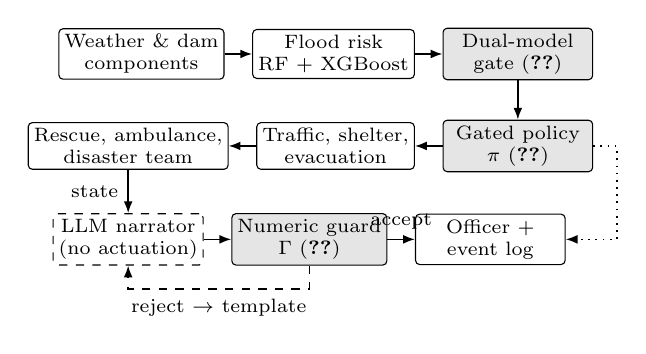
\begin{tikzpicture}[
  font=\scriptsize,
  box/.style={draw, rounded corners=1.5pt, align=center, minimum width=1.9cm, minimum height=0.58cm, inner sep=2pt},
  gate/.style={box, fill=gray!20},
  llm/.style={box, dashed},
  arr/.style={-{Latex[length=1.5mm]}, semithick}]
\node[box] (wx) {Weather \& dam\\components};
\node[box, right=0.35cm of wx] (fr) {Flood risk\\RF + XGBoost};
\node[gate, right=0.35cm of fr] (dual) {Dual-model\\gate (\ref{eq:dual})};
\node[gate, below=0.5cm of dual] (pol) {Gated policy\\$\pi$ (\ref{eq:policy})};
\node[box, left=0.35cm of pol] (ops) {Traffic, shelter,\\evacuation};
\node[box, left=0.35cm of ops] (res) {Rescue, ambulance,\\disaster team};
\node[llm, below=0.55cm of res] (llm) {LLM narrator\\(no actuation)};
\node[gate, right=0.35cm of llm] (guard) {Numeric guard\\$\Gamma$ (\ref{eq:guard})};
\node[box, right=0.35cm of guard] (hum) {Officer +\\event log};
\draw[arr] (wx) -- (fr);
\draw[arr] (fr) -- (dual);
\draw[arr] (dual) -- (pol);
\draw[arr] (pol) -- (ops);
\draw[arr] (ops) -- (res);
\draw[arr] (res) -- node[left]{state} (llm);
\draw[arr] (llm) -- (guard);
\draw[arr] (guard) -- node[above]{accept} (hum);
\draw[arr, dashed] (guard.south) -- ++(0,-0.3) -| node[pos=0.25, below]{reject $\rightarrow$ template} (llm.south);
\draw[arr, dotted] (pol.east) -- ++(0.3,0) |- (hum.east);
\end{tikzpicture}
\caption{Pipeline. Shaded blocks can only hold, downgrade or reject; none can trigger an action. The LLM (dashed) receives the shared state and has no actuation rights. The dotted link carries every policy decision and its reason to the officer.}
\label{fig:arch}
\end{figure}

\subsection{Decision Policy and Disagreement Gate}
The flood-risk component receives a flood probability $p$ and three health flags: $h_d$ (weather and river data available), $h_m$ (model loaded and returned a value) and $h_s$ (database connected). An operator can set an override $o$, and a flag $A$ enables automation. With $\tau_m=0.50$ and $\tau_a=0.60$, served from one configuration module,
\begin{equation}
\pi(p,\mathbf{h},o)=
\begin{cases}
\textsc{unavailable} & p \text{ undefined}\\
\textsc{override} & o\\
\textsc{monitor} & p<\tau_m\\
\textsc{auto} & p\ge\tau_a \wedge h_d\wedge h_m\wedge h_s\wedge A\\
\textsc{review} & \text{otherwise.}
\end{cases}
\label{eq:policy}
\end{equation}
A Random Forest \cite{Breiman2001} and an XGBoost model \cite{Chen2016}, the latter supplying $p$, were trained on the INDOFLOODS catalogue (\ClsEvents{} events at \ClsGauges{} gauges) to predict whether an event is severe (held-out ROC-AUC \ClsAucRf{} and \ClsAucXgb). Automatic dispatch is held when
\begin{multline}
H=\big[\,|p_{\mathrm{RF}}-p_{\mathrm{XGB}}|\ge\delta\,\big]\\
\vee\ \big[\min(p_{\mathrm{RF}},p_{\mathrm{XGB}})<\tau_a\le\max(p_{\mathrm{RF}},p_{\mathrm{XGB}})\big],
\label{eq:dual}
\end{multline}
with $\delta=0.15$; the second, \emph{straddle} term flags models on opposite sides of the threshold.

\subsection{LLM Narration and the Numeric Guards}
\label{sec:guards}
The band follows $p$ (calm below 0.40, watch below 0.50, administrator review below 0.60, automated response above) and sets who speaks and the tone; the action is still set by $\pi$. The prompt lists the current facts (probabilities, rainfall, river level, barrage stage, time and place), states the band's rule and tells the model to use only those numbers. The rule of the automated band reads ``Above 60\%: flood occurred'', and the template that replaces a rejected reply begins ``Flood has occurred''; Sec.~\ref{sec:claims} returns to this wording.

Let $\mathcal{N}(s)$ be the decimal numbers in a string $s$ and $F$ the prompt text up to the recent-history block. With $\tilde F=\{f,100f,f/100: f\in\mathcal{N}(F)\}$, the deployed guard accepts turns $T$ when
\begin{equation}
\Gamma(T)=\bigwedge_{t\in T}\ \bigwedge_{n\in\mathcal{N}(t)}\ \exists f\in\tilde F:\ |n-f|\le \tfrac12 10^{-d(n)},
\label{eq:guard}
\end{equation}
where $d(n)$ is the number of decimals written in $n$, so honest rounding passes. The guard is untyped: a number written as a word is invisible to it, and an integer drawn uniformly from $[a,b]$ passes with probability
\begin{equation}
P_{\mathrm{miss}}= |\{\lfloor f\rceil : f\in\tilde F\}\cap[a,b]|\,/\,(b-a+1),
\label{eq:miss}
\end{equation}
where $\lfloor f\rceil$ is the integer nearest to $f$ (the only integers within the tolerance of (\ref{eq:guard}) for $d(n)=0$).

\textit{Typed guards.} $\Gamma_{\mathrm{T}}$ reads facts from the structured state and binds each number to a quantity before checking it: number words become digits, clock times must equal the current time, a number with ``\%'' must match a model probability or a threshold of the band, one with ``mm'' the rainfall and one with ``m'' a water level. An unbound number is rejected. A revised version, $\Gamma_{\mathrm{T}}^{(2)}$, adds a list of procedural numbers (reporting intervals, deadlines given as orders), rejects every arrival time and binds a value without a unit to the quantity named just before it.

\textit{Slots-only narrator.} Instead of checking numbers, the prompt can forbid them: the model writes no digit or number word and refers to facts by placeholders (\{probability\}, \{rain\_mm\}, \{river\_m\}, \{barrage\_m\}, \{time\}, \{threshold\}, \{places\}), which the program fills from the state. A reply whose raw text contains a digit, a word from a fixed number-word lexicon $\mathcal{W}$ or an unknown placeholder is replaced by the template.

\begin{definition}[Grounded reply]
Let the state $\sigma$ assign a value $v_q$ to each quantity $q$ it holds. A \emph{numeric mention} is a number $n$ in the reply, in digits or words, together with the quantity $q$ it describes. A reply is \emph{grounded} in $\sigma$ if every mention is procedural, quotes a threshold of the current band, or has $q$ in $\sigma$ and $|n-v_q|\le\frac12 10^{-d(n)}$. It is \emph{value-grounded} if every number it contains equals some state value or threshold, whatever quantity it is attached to.
\end{definition}

\begin{proposition}[Slots-only render]
If the raw text of a slots-only reply contains no digit, no word of $\mathcal{W}$ and no unknown placeholder, and no place name contains a digit, then the rendered reply is value-grounded. It is grounded if, in addition, the model wrote each placeholder where its quantity is meant.
\end{proposition}
\begin{IEEEproof}
Every digit of the rendered text was inserted by the renderer, which writes only state values and band thresholds into known placeholders; the raw text contributes none, and no number word from $\mathcal{W}$.
\end{IEEEproof}
The guarantee has two stated gaps: number words outside $\mathcal{W}$ (``eleven'', ``a dozen'') and a placeholder put where another quantity is meant. Neither is a guard failure in the sense of (\ref{eq:guard}); both are checked empirically in Sec.~\ref{sec:design}.

\section{Evaluation Setup}
\textit{Decision path.} We evaluated (\ref{eq:policy}) on $p\in\{0,0.001,\dots,1\}$ plus an undefined value, all eight health combinations and both override states (\PolCases{} cases), against five properties (\textsc{auto} only if every check passes and $p\ge\tau_a$; undefined $p$ gives \textsc{unavailable}; $p<\tau_m$ without override gives \textsc{monitor}; $p\ge\tau_a$ with a failed check gives \textsc{review}; monotone in $p$ when healthy). We then extracted the dispatch decision into a pure function and checked the composed path (policy, hold, dispatch) for the property that teams are dispatched only when every check passes and the models agree, or an operator overrides, over \EtoECases{} cases.

\begin{lemma}[Grid coverage]
Assume (i) the extracted policy and dispatch functions read $p$ only through the comparisons $p<0.40$, $p<0.50$ and $p\ge0.60$; (ii) these thresholds are grid points and the code compares against the same binary floating-point constants that the grid produces ($k/1000$ in IEEE 754 double precision); (iii) $H$ enters the dispatch function as a free boolean, enumerated in both values for every $p$; (iv) health flags and override are booleans. Then the grid check of a property over $\{0,0.001,\dots,1\}$ decides it for every $p\in[0,1]$.
\end{lemma}
\begin{IEEEproof}
By (i), the outputs are constant on each of $[0,0.40)$, $[0.40,0.50)$, $[0.50,0.60)$ and $[0.60,1]$; by (ii), each interval contains grid points and its end points fall in the right interval; by (iii) and (iv), every other input is enumerated.
\end{IEEEproof}
The lemma covers the extracted functions. Because $H$ is a free input, the check holds for any hold the gate might output; it does not verify that (\ref{eq:dual}) computes $H$ correctly, and it says nothing about the asynchronous pipeline around the functions.

\textit{Live replies.} For \LiveStates{} seeded states (rainfall 5--250~mm in a monsoon month, both model probabilities from the deployed classifiers, river 200.0--208.5~m, barrage 199.0--206.0~m) we sent the production prompt through the Groq API to \texttt{openai/gpt-oss-20b} and \texttt{openai/gpt-oss-120b} on 10 Oct.\ 2026 (\LiveN{} replies, all parsed), without fallback, and stored every verdict. The temperature was 0.85 because that is the value the deployed narrator uses; we did not tune it. Reference labels follow a written protocol. A number is \emph{supported} if it states a state value for the quantity it describes (honest rounding allowed) or quotes a band threshold; \emph{procedural} numbers (reporting intervals, the count of named places, band ranges, deadlines given as orders) are ignored; anything else, including any arrival time, is \emph{unsupported}. A script applies the protocol; replies on which it disagreed with any checker were then read by one author, and \LiveOverrides{} labels were changed, all to ``procedural''. That reading saw the checkers' verdicts, so we also report results under the script's labels alone. Intervals resample states (2,000 replicates), since both models answer the same states.

\textit{Prompt designs.} For the first \VarStates{} states and the same models we ran on 13 Oct.\ 2026 the production prompt plus one line forbidding arrival times, and the slots-only prompt (\VarN{} calls each), plus the unchanged production prompt on the first 50 states (\VarBaseN{} calls) to check for drift. These replies were labelled by the script only.

\textit{LLM judge.} Qwen3 27B (API identifier \texttt{qwen/qwen3.8-27b}), a family different from the generators, received the structured facts and the turns at temperature 0 and returned whether every number was supported \cite{Zheng2023}, for 320 injected replies (40 states) and the \LiveN{} live replies (10--11 Oct.\ 2026). \JudFailN{} live calls failed after retries; the deployed system would send these to the template.

\textit{Held-out model family.} $\Gamma_{\mathrm{T}}^{(2)}$ was written from the misses on the development replies, frozen and hashed (SHA-256) before replies of \texttt{allam-2-7b} were collected for the same \HoStates{} states on 10 Oct.\ 2026. \HoN{} replies parsed; the other \HoParseFail{} calls, all in the automated band, failed or returned invalid JSON. Reading changed \HoOverrides{} labels, again all to ``procedural''.

\textit{Claim check.} A short pattern check rejects sentences that assert an observed flood (``flood confirmed'', ``has breached'', ``water ingress'') unless a hedge (``could'', ``chance of'', ``expected'') precedes them. It was written on the development replies and frozen by hash before any reply of the prompt-design run was read. Its accuracy has not been measured.

\section{Results}
\subsection{The Decision Path}
\label{sec:audit}
The policy satisfied all five properties in every case. The composed check found that the original dispatch step tested the probability band and the hold but never read the action returned by $\pi$: when a health check failed while both models agreed on a high probability, $\pi$ returned \textsc{review} and teams were still dispatched (\EtoEViolBefore{} grid cases, one equivalence class). In the prototype's own rainfall sweep, \SweepAutoRel{} of \SweepN{} settings were in that state. After the fix (dispatch requires \textsc{auto} or \textsc{override}, and the hold applies in both modes) the check found \EtoEViolAfter{} violations. An end-to-end test would also have caught this integration error; we report it to show that a property check on the composed path finds it systematically, and because the rest of the paper relies on it: once only $\pi$ can actuate, a wrong narration can mislead an officer but cannot dispatch a team.

\subsection{Numeric Grounding of Live Replies}
\LiveUnsup{} of the \LiveN{} replies (\LiveUnsupPct\%, 95\% interval \LiveUnsupCi\%) stated at least one unsupported number, and \LiveEta{} of these \LiveUnsup{} were invented arrival times such as ``ETA 10 minutes''; the prompt contains no ETA. Table~\ref{tab:live} compares the checks.

\begin{table}[t]
\caption{Checks on the \LiveN{} live gpt-oss replies (reference labels)}
\label{tab:live}
\centering
\footnotesize
\setlength{\tabcolsep}{2.4pt}
\begin{tabular}{lcccc}
\toprule
Check & $n$ & Recall & False rej. & Calls\\
\midrule
\input{tab_live.tex}
\bottomrule
\multicolumn{5}{l}{\scriptsize In \%, 95\% state-clustered bootstrap intervals in brackets. Recall over}\\
\multicolumn{5}{l}{\scriptsize unsupported replies, false rejections over supported ones. ``Answered}\\
\multicolumn{5}{l}{\scriptsize only'' drops the \JudFailN{} judge calls that failed. Calls: model calls per check.}\\
\end{tabular}
\end{table}

The typed guard caught more than the deployed guard but rejected \LiveTypFpN{} supported replies, mostly for procedural numbers or values without a unit (``barrage 202.26''). Its extra false rejections are clear (difference \TypDepFprDiffCi{} points); its extra recall is weaker evidence, since the exact paired test gives $p=\McDevTypRecP$ while the clustered interval of the difference is \TypDepRecDiffCi{} points. The LLM judge recognises an invented ETA in any wording, but it costs one model call per message, failed on \JudFailN{} of \LiveN{} calls, and is itself a model whose verdicts cannot be checked exhaustively. Under the script's labels alone (\PoDevUnsup{} unsupported replies instead of \LiveUnsup), the guards' recall was \PoDevDepRec\%, \PoDevTypRec\% and \PoDevVtwoRec\%.

\subsection{What the Errors Are}
Table~\ref{tab:tax} classifies every unsupported reply that we stored. Categories are assigned by keyword rules on the context of each number the labelling script flagged (for example, a number followed by ``people'' or ``affected'' is a head-count); nobody read the replies to assign them. The two development models erred almost only with arrival times, the held-out model with head-counts, durations and misquoted facts.

\begin{table}[t]
\caption{Error taxonomy over all \TaxN{} stored replies}
\label{tab:tax}
\centering
\footnotesize
\setlength{\tabcolsep}{2.2pt}
\begin{tabular}{lccccrccc}
\toprule
 & \multicolumn{4}{c}{Replies with error (\%)} & & \multicolumn{3}{c}{Passed (\%)}\\
Category & 20b & 120b & ALLaM & Var. & $n$ & $\Gamma$ & $\Gamma_{\mathrm{T}}$ & $\Gamma_{\mathrm{T}}^{(2)}$\\
\midrule
\input{tab_taxonomy.tex}
\bottomrule
\multicolumn{9}{l}{\scriptsize 20b, 120b: \LiveStates{} replies each; ALLaM: \HoN; Var.: the \TaxVarN{} prompt-design replies.}\\
\multicolumn{9}{l}{\scriptsize $n$: replies with the error. Passed: share of them a guard accepted;}\\
\multicolumn{9}{l}{\scriptsize $\Gamma_{\mathrm{T}}^{(2)}$ only on the \TaxNotDev{} replies not used to design it. A reply can fall}\\
\multicolumn{9}{l}{\scriptsize in several rows. No rate of rise was flagged.}\\
\end{tabular}
\end{table}

The deployed guard passed \TaxEtaPassDep\% of replies with an invented ETA and \TaxWordPassDep\% of those with a number word. Eq.~(\ref{eq:miss}) explains only part of this. The \EqDigitN{} development replies whose only error was an ETA in digits used \EqA--\EqB{} minutes; over that range, (\ref{eq:miss}) gives a miss probability of \EqPmissMean\% on average (at most \EqPmissMax\%) for the facts of each state, so \EqExpUni{} of these replies should pass by collision (\EqExpEmp{} with the observed distribution of values, which favours 10 and 15). \EqMeas{} did. Of the \LiveDepMiss{} development replies the deployed guard missed, the other \MissRestN{} lie outside (\ref{eq:miss}): \MissWordsN{} wrote the ETA in words, \MissClockN{} as a clock time and \MissOtherN{} contained another error. Misquoted facts are the class that every guard still passed (\TaxFactPassDep--\TaxFactPassVtwo\%); a value close to a fact for another quantity passes an untyped check, and the typed guards bind by nearby words, which a long sentence can mislead.

\subsection{Prompt Designs}
\label{sec:design}
Table~\ref{tab:design} gives the alternative prompts. Re-run on the same day, the production prompt still produced an unsupported number in \VarBaseUnsup\% of replies (\VarBaseCi\%). One added line forbidding arrival times lowered this to \VarNoetaUnsup\% (\VarNoetaCi\%) at a cost of \VarNoetaTokDiff{} tokens per call. The slots-only prompt left a digit or number word in \VarSlotsViol\% of replies, which fell back to the template.

\begin{table}[t]
\caption{Prompt designs, live, first \VarStates{} states (script labels)}
\label{tab:design}
\centering
\footnotesize
\setlength{\tabcolsep}{2.2pt}
\begin{tabular}{lccccccc}
\toprule
Prompt & Calls & Unsup. & ETA & Templ. & Claim & Tokens & Words\\
\midrule
\input{tab_design.tex}
\bottomrule
\multicolumn{8}{l}{\scriptsize Unsup., ETA, Templ., Claim in \% of replies. Templ.: replaced by the template}\\
\multicolumn{8}{l}{\scriptsize (failed call or rejected by $\Gamma$; for slots, rejected by the slot check). Claim:}\\
\multicolumn{8}{l}{\scriptsize flagged by the claim check (accuracy not measured). Tokens: prompt + output}\\
\multicolumn{8}{l}{\scriptsize per call; words per reply. $^\ast$First 50 states only.}\\
\end{tabular}
\end{table}

\VarSlotsResidWCap{} of the \SlotsPassed{} replies that passed the slot check was still flagged by the labelling script. Read against the Proposition, it is not a counterexample. The flagged number is the river level, a state value; the model wrote ``\{rain\_mm\} mm rainfall, \{river\_m\} metres river level'', which renders a doubled unit, and the script binds a number to rainfall when ``rain'' occurs just before it. The same reply wrote ``Estimated time \{time\}'', so the current time is presented as an arrival time: value-grounded, but with a placeholder where another quantity is meant, the second gap of the Proposition. A scan of the passed replies found no number word outside $\mathcal{W}$. Whether placeholder replies read as well on a radio net is a question for officers.

\subsection{Injected Errors}
On \GuardCtx{} states, each with one grounded reply and seven copies holding one wrong value, passed through the production code with the HTTP client stubbed, the deployed guard rejected \GAllDeployed\% of wrong digit strings, none of the grounded replies and none of the wrong values written in words. Its \GMissN{} misses were collisions: \GMissFact{} with a genuine fact for another quantity, \GMissRule{} with a band threshold and \GMissScale{} with a $\times100$ copy. The typed guard rejected \GAllTyped\% of wrong digit strings and \GWordsTyped\% of wrong number words. On a subset of \JudgeInjStates{} states the LLM judge was the weakest check on small probability errors, which change a single digit (it missed \JudgeProbSmallMiss\%).

\subsection{A Held-Out Model Family}
\label{sec:heldout}
Table~\ref{tab:heldout} separates the development replies, on which $\Gamma_{\mathrm{T}}^{(2)}$ was built and is perfect by construction, from the frozen test on ALLaM-2. \HoUnsup{} of its \HoN{} replies (\HoUnsupPct\%) were unsupported, with the error mix of Table~\ref{tab:tax}. The frozen guard caught \HoVtwoRec\% against \HoDepRec\% for the deployed guard, a difference of \HoDiffW{} replies (McNemar $p=\McVtwoRecP$; clustered interval \HoVtwoDepRecDiffCi{} points), and rejected \HoVtwoFp{} correct replies against \HoDepFp, all of them procedural labels such as ``Team 1'' that the development models never wrote. On this set neither guard is shown to be better. Under the script's labels, which count those labels as unsupported, neither guard falsely rejected any held-out reply, which shows how much false-rejection rates depend on the procedural judgement.

\begin{table}[t]
\caption{Guards on development replies and on a held-out model family}
\label{tab:heldout}
\centering
\footnotesize
\setlength{\tabcolsep}{2.2pt}
\begin{tabular}{lcccc}
\toprule
 & \multicolumn{2}{c}{gpt-oss, $n=\LiveN$} & \multicolumn{2}{c}{ALLaM-2, $n=\HoN$ (held out)}\\
Check & Recall & False rej. & Recall & False rej.\\
\midrule
\input{tab_heldout.tex}
\bottomrule
\multicolumn{5}{l}{\scriptsize In \%, 95\% bootstrap intervals over states. $\Gamma_{\mathrm{T}}^{(2)}$ was frozen by hash}\\
\multicolumn{5}{l}{\scriptsize before any ALLaM-2 reply was read.}\\
\end{tabular}
\end{table}

Table~\ref{tab:ablation} removes one component of $\Gamma_{\mathrm{T}}^{(2)}$ at a time. The ETA ban carries most of the recall on the development models and on the prompt-design replies (\AbVarUnsup{} unsupported of \TaxVarN, also unseen when the guard was frozen); the clock rule matters only on the held-out model; the procedural list prevents false rejections and catches nothing; unit binding changed no verdict on any set. On the prompt-design replies the frozen guard caught \AbFullVarRec\%, below its development score.

\begin{table}[t]
\caption{Ablation of $\Gamma_{\mathrm{T}}^{(2)}$: recall / false rejections (\%)}
\label{tab:ablation}
\centering
\footnotesize
\setlength{\tabcolsep}{2.6pt}
\begin{tabular}{lcccccc}
\toprule
 & \multicolumn{2}{c}{gpt-oss (dev.)} & \multicolumn{2}{c}{ALLaM-2} & \multicolumn{2}{c}{Prompt designs}\\
Guard & Rec. & FR & Rec. & FR & Rec. & FR\\
\midrule
\input{tab_ablation.tex}
\bottomrule
\multicolumn{7}{l}{\scriptsize ``--'': component switched off. Labels: reference (dev., ALLaM-2), script (designs).}\\
\end{tabular}
\end{table}

In deployment a guard's rejections become template fallbacks: \FbTwenty\% of gpt-oss-20b calls, \FbOneTwenty\% of gpt-oss-120b and \FbAllam\% of ALLaM-2 calls ended in the template.

\subsection{Qualitative Over-Claims}
\label{sec:claims}
\OcDev{} development replies (\OcDevPct\%), all in the automated band, asserted that a flood ``is confirmed'' or that water ``has breached'', although the state holds only a probability. No numeric check is designed to see them: the deployed guard passed \OcDevPassDep{} of the \OcDev, and the judge \OcDevPassJud. The wording comes partly from our own prompt, whose automated-band rule says ``flood occurred'', and the deployed template says ``Flood has occurred'', so the fallback itself over-claims. The frozen claim check flagged \VarBaseClaim\%, \VarNoetaClaim\% and \VarSlotsClaim\% of the replies to the three prompts of Table~\ref{tab:design}, which it had never seen; how many of these flags are correct, and how many over-claims it misses, has not been measured. Our grounding claim is therefore limited to numbers.

\subsection{The Disagreement Gate}
On the \CalTest{} held-out events of the classifiers' split, the deployed gate held \GateDepHold\% of events and caught \GtDepCaught{} of the policy model's \GtErrN{} errors (\GtDepRecall\%); the straddle term alone caught \GtStRecall\%. We compared the gate with a single isotonic-calibrated XGBoost model without a gate, whose threshold is set on training folds for each cost ratio. With a false dispatch costing 1, a review 0.2 and the officer assumed always right, the gate was cheaper than no gate at every ratio from 1 to 10, and cheaper than the calibrated model while a missed dispatch costs less than \BeR{} false dispatches (95\% interval \BeLo--\BeHi). The gate catches errors, but its net benefit depends on cost ratios that must be set operationally.

\section{Discussion and Limitations}
All four faults we found lay at interfaces between components. A dispatch step bypassed a verified policy, a gate tolerance was never related to the calibration of the models it compares, an untyped guard treated every number as interchangeable, and the template meant to absorb failures carried its own over-claim. A guard tuned on one model's errors met a different mix on the next. A fail-closed fallback masks the failures it absorbs unless its rate is monitored: while we prepared this study, retired API models and a token budget too small for reasoning models silently sent every reply to the template, which only the fallback rate revealed.

All rates come from one prompt family, \LiveStates{} states, temperature 0.85 and three open-weight models from two families; no frontier model was tested. Reference labels were assigned by one author, who saw the checkers' verdicts when reading disagreements; replies on which all checks agreed were not read, and the claim check has no measured precision or recall. Blind labelling sheets for both gaps are prepared, and their scores are the main open item. The error categories come from keyword rules, not from reading. River and barrage values were sampled from operating ranges, not recorded events. The decision-path lemma covers extracted functions, not the asynchronous pipeline. The gate's costs are assumptions, and no officer has used the system in an exercise.

For a deployment we draw four rules. Prefer a narrator that does not write numbers, or failing that forbid the quantities the state lacks. Speak of probabilities in prompts and templates, and check assertion words as well as numbers. Monitor the template-fallback rate per model. And re-run a labelled held-out test whenever the model behind the API changes.

\section{Conclusion}
In a flood-response pipeline where deterministic rules decide and an LLM narrates, \LiveUnsupPct\% of live replies of two open-weight models stated an unsupported number, nearly all invented arrival times; the deployed guard caught \LiveDepRec\% of them, and its misses on digit arrival times are close to the number that (\ref{eq:miss}) predicts. A narrator that writes only placeholders is grounded by construction within a stated lexicon, and its one flagged reply in \SlotsPassed{} fits the Proposition's second gap. A revised guard frozen before a third model family was queried met different errors there and was not significantly better. Qualitative over-claims, partly seeded by our own prompt and template, escape every numeric check. Our results support LLM narration only outside the decision path, with both numeric and claim checks against the state.

\section*{Acknowledgment}
The authors thank the INDOFLOODS dataset authors and Open-Meteo for openly available data.
In line with the IEEE policy on AI-generated content, the authors disclose that Claude (Anthropic) was used to help edit and restructure the text of all sections and to draft the experiment and plotting scripts. All experiments use the authors' own software and can be reproduced with fixed seeds; the live LLM replies are stored with the scripts. The authors checked every number, claim and reference and take full responsibility for the content.

\balance
\begin{thebibliography}{00}
\bibitem{Ji2023} Z. Ji \textit{et al.}, ``Survey of hallucination in natural language generation,'' \textit{ACM Comput. Surv.}, vol. 55, no. 12, Art. no. 248, 2023, doi: 10.1145/3571730.
\bibitem{Yao2023} S. Yao \textit{et al.}, ``ReAct: Synergizing reasoning and acting in language models,'' in \textit{Proc. Int. Conf. Learn. Represent. (ICLR)}, 2023.
\bibitem{Wu2024} Q. Wu \textit{et al.}, ``AutoGen: Enabling next-gen LLM applications via multi-agent conversation,'' in \textit{Proc. Conf. Lang. Model. (COLM)}, 2024.
\bibitem{Parasuraman2000} R. Parasuraman, T. B. Sheridan, and C. D. Wickens, ``A model for types and levels of human interaction with automation,'' \textit{IEEE Trans. Syst., Man, Cybern. A, Syst. Humans}, vol. 30, no. 3, pp. 286--297, 2000, doi: 10.1109/3468.844354.
\bibitem{Leveson2011} N. G. Leveson, \textit{Engineering a Safer World: Systems Thinking Applied to Safety}. Cambridge, MA, USA: MIT Press, 2011.
\bibitem{CAP2010} OASIS, ``Common Alerting Protocol version 1.2,'' OASIS Standard, Jul. 2010.
\bibitem{WangL2024} L. Wang \textit{et al.}, ``A survey on large language model based autonomous agents,'' \textit{Front. Comput. Sci.}, vol. 18, no. 6, Art. no. 186345, 2024, doi: 10.1007/s11704-024-40231-1.
\bibitem{Lewis2020} P. Lewis \textit{et al.}, ``Retrieval-augmented generation for knowledge-intensive NLP tasks,'' in \textit{Adv. Neural Inf. Process. Syst. 33}, 2020, pp. 9459--9474.
\bibitem{Min2023} S. Min \textit{et al.}, ``FActScore: Fine-grained atomic evaluation of factual precision in long form text generation,'' in \textit{Proc. Conf. Empir. Methods Nat. Lang. Process. (EMNLP)}, 2023, pp. 12076--12100, doi: 10.18653/v1/2023.emnlp-main.741.
\bibitem{Manakul2023} P. Manakul, A. Liusie, and M. J. F. Gales, ``SelfCheckGPT: Zero-resource black-box hallucination detection for generative large language models,'' in \textit{Proc. Conf. Empir. Methods Nat. Lang. Process. (EMNLP)}, 2023, pp. 9004--9017, doi: 10.18653/v1/2023.emnlp-main.557.
\bibitem{Dhuliawala2024} S. Dhuliawala \textit{et al.}, ``Chain-of-verification reduces hallucination in large language models,'' in \textit{Findings Assoc. Comput. Linguist. (ACL)}, 2024, pp. 3563--3578, doi: 10.18653/v1/2024.findings-acl.212.
\bibitem{Zheng2023} L. Zheng \textit{et al.}, ``Judging LLM-as-a-judge with MT-Bench and Chatbot Arena,'' in \textit{Adv. Neural Inf. Process. Syst. 36}, 2023, pp. 46595--46623, doi: 10.52202/075280-2020.
\bibitem{Rebedea2023} T. Rebedea, R. Dinu, M. N. Sreedhar, C. Parisien, and J. Cohen, ``NeMo Guardrails: A toolkit for controllable and safe LLM applications with programmable rails,'' in \textit{Proc. Conf. Empir. Methods Nat. Lang. Process.: Syst. Demonstrations}, 2023, pp. 431--445, doi: 10.18653/v1/2023.emnlp-demo.40.
\bibitem{Zhang2025} Y. Zhang, S. Y. Emma, A. L. J. En, and J. S. Dong, ``RvLLM: LLM runtime verification with domain knowledge,'' in \textit{Adv. Neural Inf. Process. Syst. 38}, 2025, pp. 89374--89394, doi: 10.52202/085713-2693.
\bibitem{WangH2026} H. Wang, C. M. Poskitt, and J. Sun, ``AgentSpec: Customizable runtime enforcement for safe and reliable LLM agents,'' in \textit{Proc. IEEE/ACM 48th Int. Conf. Softw. Eng. (ICSE)}, 2026, pp. 2938--2950, doi: 10.1145/3744916.3764546.
\bibitem{Wiseman2017} S. Wiseman, S. Shieber, and A. Rush, ``Challenges in data-to-document generation,'' in \textit{Proc. Conf. Empir. Methods Nat. Lang. Process. (EMNLP)}, 2017, pp. 2253--2263, doi: 10.18653/v1/D17-1239.
\bibitem{Thomson2020} C. Thomson and E. Reiter, ``A gold standard methodology for evaluating accuracy in data-to-text systems,'' in \textit{Proc. 13th Int. Conf. Nat. Lang. Gener. (INLG)}, 2020, pp. 158--168, doi: 10.18653/v1/2020.inlg-1.22.
\bibitem{Kasner2024} Z. Kasner and O. Du\v{s}ek, ``Beyond traditional benchmarks: Analyzing behaviors of open LLMs on data-to-text generation,'' in \textit{Proc. 62nd Annu. Meeting Assoc. Comput. Linguist. (ACL)}, 2024, pp. 12045--12072, doi: 10.18653/v1/2024.acl-long.651.
\bibitem{Wen2015} T.-H. Wen, M. Ga\v{s}i\'{c}, N. Mrk\v{s}i\'{c}, P.-H. Su, D. Vandyke, and S. Young, ``Semantically conditioned LSTM-based natural language generation for spoken dialogue systems,'' in \textit{Proc. Conf. Empir. Methods Nat. Lang. Process. (EMNLP)}, 2015, pp. 1711--1721, doi: 10.18653/v1/D15-1199.
\bibitem{Alshiekh2018} M. Alshiekh, R. Bloem, R. Ehlers, B. K\"{o}nighofer, S. Niekum, and U. Topcu, ``Safe reinforcement learning via shielding,'' in \textit{Proc. AAAI Conf. Artif. Intell.}, vol. 32, no. 1, 2018, pp. 2669--2678, doi: 10.1609/aaai.v32i1.11797.
\bibitem{Lakshminarayanan2017} B. Lakshminarayanan, A. Pritzel, and C. Blundell, ``Simple and scalable predictive uncertainty estimation using deep ensembles,'' in \textit{Adv. Neural Inf. Process. Syst. 30}, 2017, pp. 6402--6413.
\bibitem{Breiman2001} L. Breiman, ``Random forests,'' \textit{Mach. Learn.}, vol. 45, no. 1, pp. 5--32, 2001, doi: 10.1023/A:1010933404324.
\bibitem{Chen2016} T. Chen and C. Guestrin, ``XGBoost: A scalable tree boosting system,'' in \textit{Proc. 22nd ACM SIGKDD Int. Conf. Knowl. Discov. Data Min.}, 2016, pp. 785--794, doi: 10.1145/2939672.2939785.
\end{thebibliography}

\end{document}
